% ---------------------------------------------------------------------------
% paper_supplement.tex -- self-contained, compilable document that assembles the
% new Methodology / Results / Analysis sections with their figures, so the work
% can be read as one PDF.
%
% Build (from the paper/ directory):
%     pdflatex paper_supplement.tex
%     pdflatex paper_supplement.tex      % second pass resolves \ref cross-refs
%
% Figures live in ../experiments/plots/ (set via \graphicspath below). They are
% PNGs, which pdflatex embeds directly.
%
% This is a *reading/preview* wrapper. To fold the content into the main paper,
% \input the three fragment files directly and delete this wrapper's preamble.
% ---------------------------------------------------------------------------
\documentclass[11pt]{article}

\usepackage[T1]{fontenc}
\usepackage[utf8]{inputenc}
\usepackage[margin=1in]{geometry}
\usepackage{booktabs}
\usepackage{graphicx}
\usepackage{amsmath}
\usepackage[hidelinks]{hyperref}

% Figures are one directory up, under experiments/plots/.
\graphicspath{{../experiments/plots/}}

% Absorb the few points-too-wide lines (long \texttt{} tokens) without rewording.
\emergencystretch=3em

\title{AES Cache-Timing Laboratory:\\
       Trace-Threshold, Cross-Language, and Dial-Sweep Results\\
       \large(supplement to draft~1 --- Results and Analysis)}
\author{}
\date{}

\begin{document}
\maketitle

\noindent\emph{This supplement extends the draft (Introduction + Methodology)
with the experiments actually run: the C trace-count threshold, the native
cross-language recovery comparison (C vs.\ Go), the Go garbage-collector
ablation, and the dial sweep. Numbering here is local to the supplement; when
merged into the main paper the section/figure/table numbers will renumber
automatically.}

\bigskip

% --- Methodology additions (subsections; attach under the main Section 2) ------
% Numbered \section so the \subsection fragments render as 1.1, 1.2, ... rather
% than 0.1 under an unnumbered heading.
\section{Methodology additions}
% Methodology additions -- drop-in fragment for the paper.
% Requires: \usepackage{booktabs}. Slots after the existing Section 2.
% These subsections extend the draft's Methodology to cover the experiments
% that were actually run (dial sweep, native cross-language collection, and the
% garbage-collector ablation) and record the dataset-governance rules.

\subsection{Dial Sweep at a Fixed Trace Count}
\label{sec:method-dial}
The threshold experiment varies trace count while holding the two collection
``dials'' fixed. A complementary experiment holds trace count fixed and varies
the dials, to separate the contribution of \emph{averaging} from that of
\emph{signal strength}:
\begin{itemize}
  \item \texttt{-repeat} $r$: the number of vulnerable encryptions accumulated
        into one trace. Larger $r$ raises the target operation's contribution
        relative to fixed timer overhead (more averaging per trace).
  \item \texttt{-evict-kb} $e$: the size of the memory region read before each
        timed operation. Larger $e$ disturbs more of the cache and is expected
        to strengthen the collision signal.
\end{itemize}
The count is fixed at \textbf{100{,}000 traces}. This value is chosen
deliberately: it sits in the C attack's \emph{marginal} region, just above its
50\% threshold (Section~\ref{sec:results-threshold}), where recovery is most
sensitive to changes in signal quality. A count deep in the reliable regime
(where recovery is already~100\%) or deep in the failure regime (0\%) would
mask any dial effect; the knee maximises the visible dynamic range. We sweep
$r \in \{10,20,30,50,75,100\}$ and $e \in \{256,512,1024,2048,4096\}$~KiB, each
about the $r=50$, $e=2048$ baseline, with ten interleaved trials per point.

\subsection{Native Cross-Language Recovery}
\label{sec:method-crosslang}
The draft's cross-language plan (Section~2.11) supplies \emph{one shared trace
file} to C, Go, and Python to test algorithmic consistency and processing time.
The experiments reported here answer a different question. Each implementation
performs its \emph{own} measured collection with its native timer and then runs
its own recovery, and we compare the resulting \emph{recovery reliability} as a
function of trace count. This measures how each language's runtime affects the
quality of the timing channel it can capture---the ``separate runtime-dependent
experiment'' the draft anticipates---rather than the correctness of a shared
computation.

Because each language collects independently, the trace data (and its random
seed) differ across implementations. Trace count, the fixed AES key, the dial
settings, the outlier rule, the recovery algorithm, and the verification
criterion are held identical; only the implementation (and hence its collection
runtime) changes. Differences in recovery are therefore attributable to the
language's runtime behaviour during collection, not to the attack logic, which
is common. We treat this as a \emph{native-collection} comparison and keep it
distinct from the shared-dataset consistency test, which remains future work.

\subsection{Garbage-Collector Ablation (Go)}
\label{sec:method-gc}
Go executes within a managed runtime whose garbage collector (GC) and goroutine
scheduler can preempt execution at unpredictable moments, adding jitter to the
per-trace timings the attack depends on. To test whether this runtime noise is
the cause of Go's higher threshold, we repeat the Go collection with two
environment settings that quiet the runtime without altering the attack:
\texttt{GOGC=off} (disables the collector, so no GC pause lands inside a timed
region) and \texttt{GOMAXPROCS=1} (pins execution to one core, suppressing
cross-core migration). Both are read by the Go runtime from the environment; no
source change is made. For cost reasons the ablation uses a reduced grid (counts
$\{500{,}000, 250{,}000, 100{,}000, 50{,}000\}$ and a $3\times3$ dial grid), so
it is compared to the garbage-collected run only at matched points and by the
fitted 50\% threshold, never by a grid-dependent high-reliability count.

\subsection{Dataset Governance and Exclusion Criteria}
\label{sec:method-governance}
Several exploratory runs preceded the retained runs. To avoid selective
reporting, inclusion follows fixed rules, and every excluded run's metadata is
preserved (see the provenance table).
\begin{itemize}
  \item \textbf{Environment gate.} A run is excluded if its mean collection cost
        exceeds roughly $1.2$~ms/sample (baseline $\approx 0.94$), a proxy for
        background load. One 10-trial C sweep is excluded on this basis
        ($\approx 3.0$~ms/sample, threefold inflated).
  \item \textbf{Design gate.} Pilot runs with fewer trials, missing
        reproducibility sidecars, or single-point grids are excluded from the
        primary analysis and used only for design context.
  \item \textbf{Implementation identity.} One retained C run was launched with an
        \texttt{IMPL=go} tag before the harness supported language selection;
        the C binary in fact executed. It is verified as C (no \texttt{impl}
        field in its metadata; \texttt{min\_time} and ms/sample matching C) and
        relabelled accordingly. This mislabelling is documented because an
        earlier positional (rather than by-name) parse of the result column
        produced incorrect tallies; all reported counts are recomputed by column
        name.
\end{itemize}


% --- Results ------------------------------------------------------------------
% Results -- drop-in fragment. Requires \usepackage{booktabs,graphicx}.
% Figures referenced live in experiments/plots/ (copy/point \includegraphics as needed).

\section{Results}
\label{sec:results}

\subsection{Trace-Count Threshold (C)}
\label{sec:results-threshold}
Table~\ref{tab:c-threshold} reports, for the canonical C run, the verified
recovery rate at each trace count with 95\% Wilson score intervals. Recovery
rises from~0\% at $\le 35$k to a reliable~100\% at $\ge 100$k. Fitting a logistic
model in $\log_2(\text{count})$ places the 50\% threshold at
$N_{50} \approx 51{,}346$ traces ($2^{15.65}$); a model-independent linear
interpolation agrees at $\approx 50{,}000$ ($2^{15.61}$). The attack first
reaches high reliability ($\ge 90\%$) at $\approx 75$k traces
(Fig.~\ref{fig:c-success}).

\begin{figure}[t]
\centering
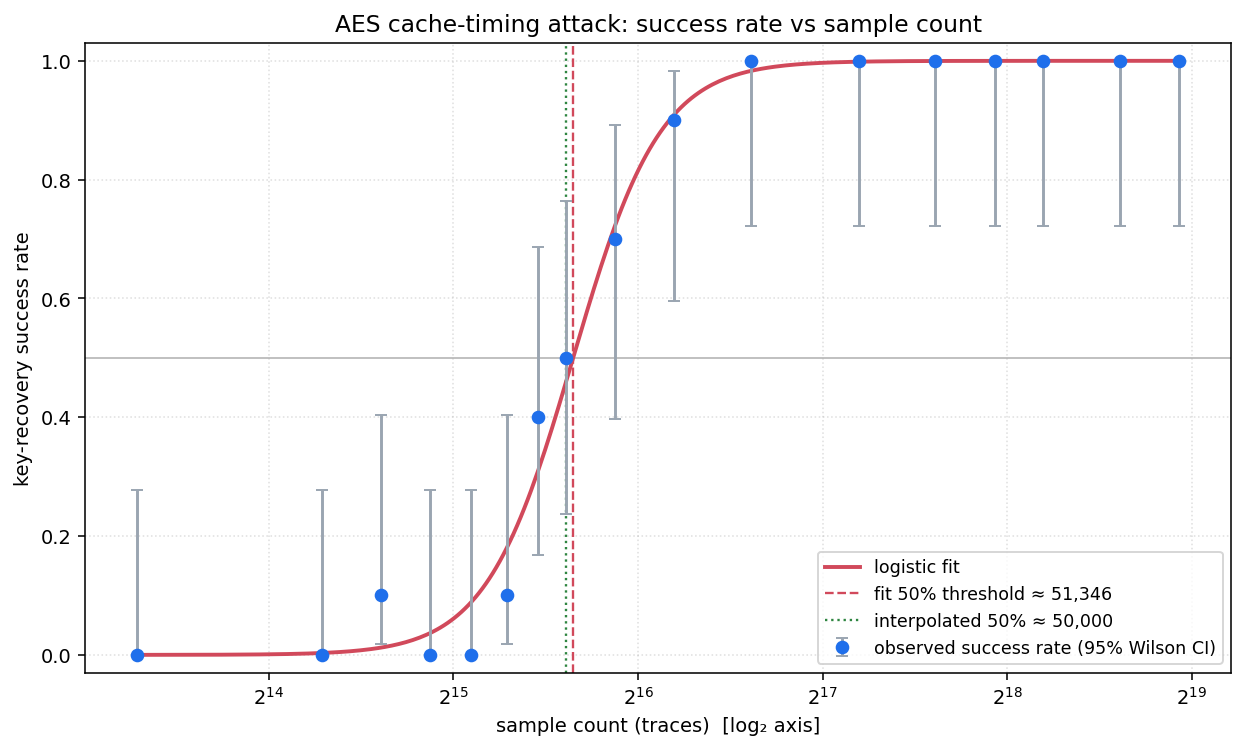
\includegraphics[width=0.85\linewidth]{go_10x_success_rate.png}
\caption{C key-recovery success rate vs.\ trace count (log$_2$ axis) with 95\%
Wilson intervals, the fitted logistic curve, and the 50\% threshold
($N_{50}\approx 51{,}346$).}
\label{fig:c-success}
\end{figure}

\begin{table}[t]
\centering
\caption{C recovery rate vs.\ trace count (canonical run; 10 trials each,
95\% Wilson CI). $N_{50}\approx 51{,}346$.}
\label{tab:c-threshold}
\begin{tabular}{rccc}
\toprule
Traces & Recovered & Rate & 95\% CI \\
\midrule
$\ge 100{,}000$ & 10/10 & 100\% & [72, 100] \\
75{,}000 & 9/10 & 90\% & [60, 98] \\
60{,}000 & 7/10 & 70\% & [40, 89] \\
50{,}000 & 5/10 & 50\% & [24, 76] \\
45{,}000 & 4/10 & 40\% & [17, 69] \\
40{,}000 & 1/10 & 10\% & [2, 40] \\
$\le 35{,}000$ & 0--1/10 & $\le$10\% & [0, 40] \\
\bottomrule
\end{tabular}
\end{table}

Across all counts the mean \texttt{min\_time} stays within 112--121 ticks and
the mean attack score within $\approx 17{,}200$--$17{,}460$ (Fig.~\ref{fig:covar}).
Neither trends with count: the per-trace leak is unchanged, and what improves
with more traces is only the stability of the group-mean estimates. The
threshold is thus a statistical (averaging) effect, not a signal cliff.

\begin{figure}[t]
\centering
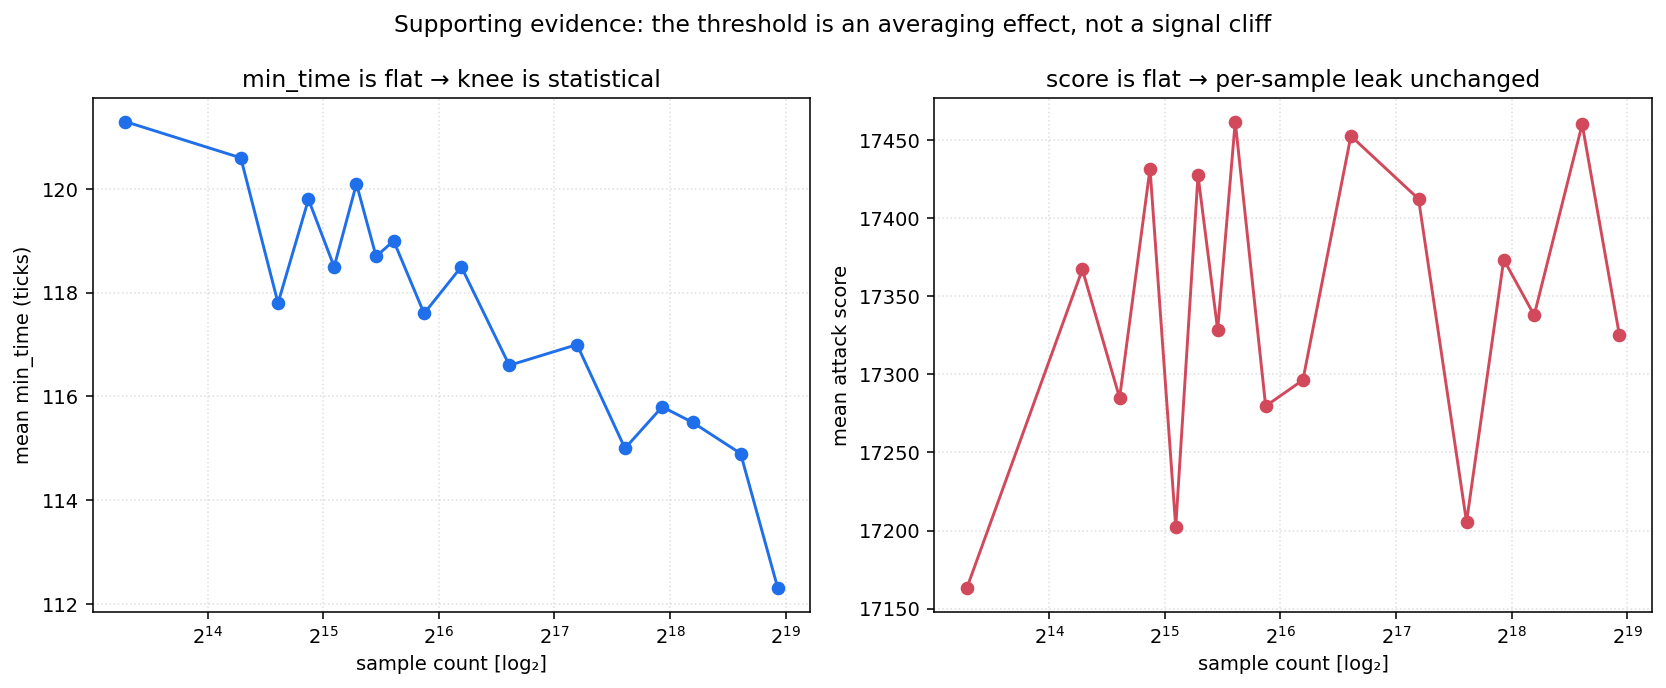
\includegraphics[width=\linewidth]{go_10x_covariates.png}
\caption{Supporting evidence: mean \texttt{min\_time} (left) and mean attack
score (right) are flat across trace count, so the per-trace leak is unchanged and
the threshold reflects averaging quality rather than a signal cliff.}
\label{fig:covar}
\end{figure}

\subsection{Cross-Language Recovery}
\label{sec:results-crosslang}
Under identical counts, key, dials, and recovery logic, the three
implementations reach 50\% recovery at very different trace counts
(Table~\ref{tab:crosslang}, Fig.~\ref{fig:crosslang}). Go requires
$N_{50}\approx 265{,}283$ ($2^{18.0}$) with the garbage collector enabled---about
$5.2\times$ the C threshold. Python is deferred (native collection at these
counts is prohibitively slow and expected to recover near~0; see limitations).

\begin{table}[t]
\centering
\caption{Fitted 50\% trace threshold by implementation (identical parameters).}
\label{tab:crosslang}
\begin{tabular}{lccc}
\toprule
Implementation & $N_{50}$ (traces) & $\log_2 N_{50}$ & Ratio to C \\
\midrule
C                 & 51{,}346  & 15.65 & 1.0$\times$ \\
Go (GC on)        & 265{,}283 & 18.02 & 5.2$\times$ \\
Go (GC off)       & 243{,}335 & 17.89 & 4.7$\times$ \\
\bottomrule
\end{tabular}
\end{table}

\begin{figure}[t]
\centering
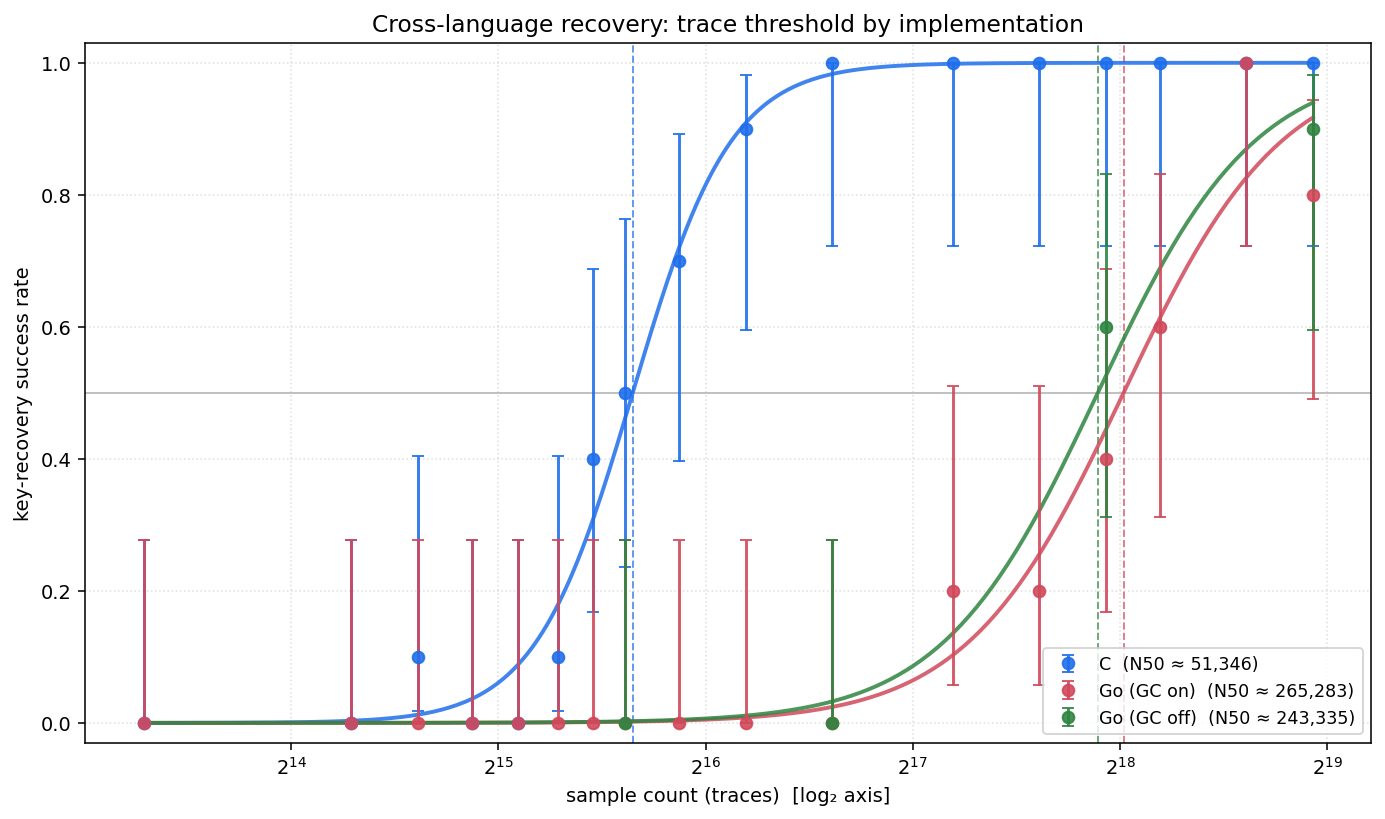
\includegraphics[width=\linewidth]{cross_language_recovery.png}
\caption{Cross-language recovery. C (blue) reaches 50\% recovery near 50k traces;
Go with the garbage collector on (red) and off (green) require roughly five times
as many, their curves nearly coincident. Points show 95\% Wilson intervals;
dashed lines mark each fitted $N_{50}$.}
\label{fig:crosslang}
\end{figure}

\subsection{Runtime-Noise Ablation (Go GC on vs.\ off)}
\label{sec:results-gc}
Disabling the Go garbage collector and pinning to one core lowers the fitted
threshold only marginally, from $N_{50}\approx 265$k to $\approx 243$k
($\approx 8\%$), well inside the sampling uncertainty. At matched counts the
GC-off run is equal or slightly better everywhere (Table~\ref{tab:gc}), but the
$\approx 5\times$ gap to C is essentially untouched. Quieting the runtime helps
a little; it does not explain Go's disadvantage.

\begin{table}[t]
\centering
\caption{Go recovery at matched counts, garbage collector on vs.\ off
(10 trials each).}
\label{tab:gc}
\begin{tabular}{rcc}
\toprule
Traces & GC on & GC off \\
\midrule
500{,}000 & 8/10 & 9/10 \\
250{,}000 & 4/10 & 6/10 \\
100{,}000 & 0/10 & 0/10 \\
50{,}000  & 0/10 & 0/10 \\
\bottomrule
\end{tabular}
\end{table}

\subsection{Dial Sweep}
\label{sec:results-dial}
At the fixed 100k count, the C dial sweep (Table~\ref{tab:dial}) shows that
increasing \texttt{-repeat} beyond the $r=50$ baseline does \emph{not} improve
recovery and appears to reduce it (70\% at $r=50$ vs.\ 20\% at $r=75,100$),
while the strongest cache disturbance, $e=4096$~KiB, gives the highest recovery
(100\%). The individual points carry wide intervals ($n=10$); the robust reading
is that signal strength (\texttt{-evict-kb}) matters more than additional
averaging (\texttt{-repeat}) at this count (Fig.~\ref{fig:dial}).

The Go dial sweep is uninformative by construction: 100k traces lie far below
Go's $\approx 265$k threshold, so recovery is $\approx 0$ (1/110 with GC on,
1/60 with GC off) regardless of dial setting. This is a consequence of fixing
the dial count at C's knee, which is below Go's operating point---a design
observation, not a null effect (Section~\ref{sec:analysis-dial}).

\begin{table}[t]
\centering
\caption{C dial sweep at 100k traces (10 trials each). Left: \texttt{-repeat}
at $e=2048$. Right: \texttt{-evict-kb} at $r=50$.}
\label{tab:dial}
\begin{tabular}{rc@{\hskip 2em}rc}
\toprule
\texttt{-repeat} & Rate & \texttt{-evict-kb} & Rate \\
\midrule
10  & 60\% & 256  & 80\%  \\
20  & 50\% & 512  & 60\%  \\
30  & 50\% & 1024 & 10\%  \\
50  & 70\% & 2048 & 50\%  \\
75  & 20\% & 4096 & 100\% \\
100 & 20\% &      &       \\
\bottomrule
\end{tabular}
\end{table}

\begin{figure}[t]
\centering
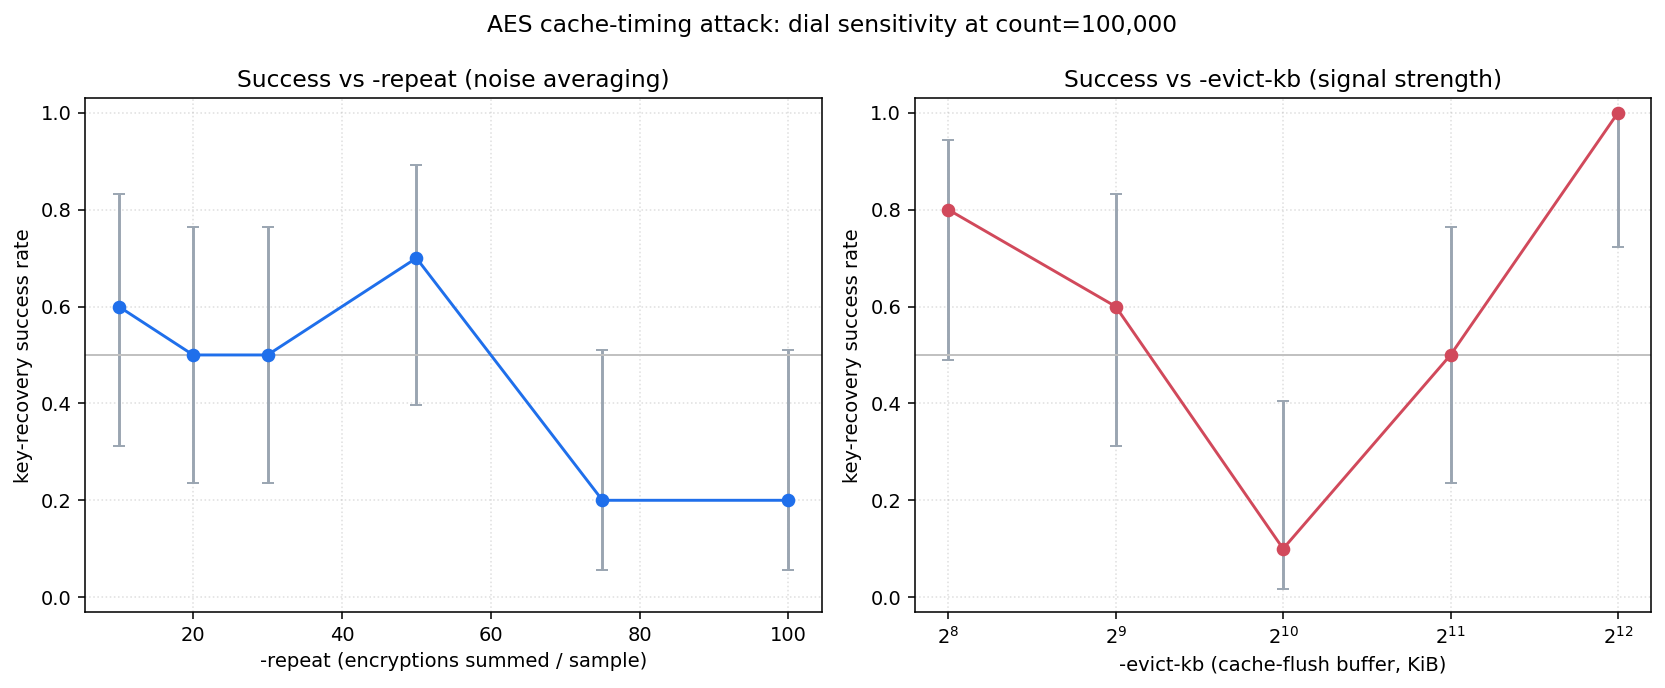
\includegraphics[width=\linewidth]{knee100k_dials.png}
\caption{C dial sweep at 100k traces: recovery rate vs.\ \texttt{-repeat} (left)
and vs.\ \texttt{-evict-kb} (right), with 95\% Wilson intervals. Stronger cache
eviction raises recovery; additional repetition does not.}
\label{fig:dial}
\end{figure}


% --- Analysis -----------------------------------------------------------------
% Analysis / Discussion -- drop-in fragment. Requires \usepackage{booktabs}.

\section{Analysis}
\label{sec:analysis}

\subsection{The Threshold Is an Averaging Effect}
\label{sec:analysis-statistical}
The flatness of \texttt{min\_time} and score across trace count
(Section~\ref{sec:results-threshold}) localises the mechanism. The per-trace
cache-collision signal---the small timing difference the attack exploits---is a
fixed quantity that does not depend on how many traces are collected. What
changes with count is the variance of each group mean $T_{i,j}[d]$: with more
traces per ciphertext-difference group, the correct final-round relation
separates from the noise floor more reliably. Recovery is therefore governed by
whether the group-mean estimates are stable enough to rank the correct relation
first, which is a smooth, probabilistic function of count---hence the
psychometric curve rather than a hard boundary.

\subsection{Why Go Needs About Five Times More Traces}
\label{sec:analysis-crosslang}
The same attack, on the same key, recovers with $\approx 5\times$ more traces in
Go than in C. Because the recovery logic is common, the difference originates in
collection: Go's measured timings are a noisier estimate of the same underlying
signal, so more traces are needed to average that noise down to the level where
the correct relation wins. The garbage-collector ablation
(Section~\ref{sec:results-gc}) sharpens this. If GC pauses were the dominant
noise source, disabling the collector would move the threshold substantially;
instead it moves $N_{50}$ by only $\approx 8\%$ and leaves the gap to C intact.
The residual noise is therefore not the collector but the broader managed-runtime
measurement path---bounds-checked array access, scheduler quanta, and coarser or
higher-overhead timing than the C collector. In short: Go's disadvantage is
real, reproducible, and a property of \emph{measurement}, not of the algorithm
or of the garbage collector specifically.\footnote{Absolute \texttt{min\_time}
values are far larger in Go than in C; whether that reflects timer units or true
overhead requires inspecting each collector's timing primitive, so we base the
cross-language claim on recovery reliability rather than on raw timing
magnitudes.}

\subsection{Dials: Signal Strength over Averaging, and a Design Lesson}
\label{sec:analysis-dial}
Within C at the 100k knee, additional \texttt{-repeat} does not help and the
largest \texttt{-evict-kb} helps most. This is consistent with the
averaging/signal split above: at a count near the threshold, the binding
constraint is the strength of the per-trace collision signal (improved by
stronger cache eviction), not additional per-trace averaging---and very large
\texttt{-repeat} may even lengthen each measurement enough to admit more
environmental perturbation. The Go dial sweep carries a methodological lesson
rather than a result: fixing the dial-sweep count at C's knee (100k) placed it
below Go's operating threshold ($\approx 265$k), so the sweep could not probe
Go's dial sensitivity. A per-implementation dial count, chosen relative to each
implementation's own threshold, would be required to compare dial effects across
languages.

\subsection{Positioning Against Prior Work}
\label{sec:analysis-priorwork}
The implemented attack follows the final-round cache-collision model of Bonneau
and Mironov, whose expanded final-round attack recovers a key from a median of
$2^{13}$--$2^{14.3}$ samples under cache eviction on 2006-era processors. Our C
threshold ($N_{50}\approx 2^{15.6}$; high-reliability $\approx 2^{16.2}$) is
roughly one order of magnitude higher. This is expected rather than
contradictory: the comparison mixes algorithm with platform and instrumentation.
Their figures use hardware cycle counters on a Pentium III/UltraSPARC, whereas
this laboratory records aggregate wall-clock time on an Apple M4 with a very
different cache hierarchy and timing resolution. The agreement to within an order
of magnitude, on entirely different hardware and with a coarser timer, indicates
that the leakage mechanism reproduces as predicted; the absolute count is a
property of this platform and instrument, not a universal constant.

\subsection{Threats to Validity}
\label{sec:analysis-threats}
\begin{itemize}
  \item \textbf{Single key.} All runs reuse one fixed AES key to isolate trace
        count; thresholds may vary across keys.
  \item \textbf{Sampling uncertainty.} Ten trials per count yield wide Wilson
        intervals, especially near 0/10 and 10/10; individual dial points should
        not be over-interpreted, and $N_{50}$ is an estimate, not a sharp value.
  \item \textbf{Run-to-run environment sensitivity.} Two clean C sweeps place the
        threshold near 50k and 100k respectively, and a contaminated sweep near
        150k; the threshold is sensitive to background load, which we control by
        the environment gate but cannot eliminate on a general-purpose machine.
  \item \textbf{Native-collection confound.} The cross-language comparison uses
        each language's own traces (different seeds), so it measures
        runtime-in-collection, not shared-dataset algorithmic consistency;
        the latter (draft RQ2) and stage-level processing time (RQ3) remain
        future work.
  \item \textbf{Reduced Go(GC-off) grid and platform confound.} The ablation uses
        a coarse count grid, and the prior-work comparison spans different
        hardware eras; both are stated where the numbers are used.
\end{itemize}


\end{document}
